\chapter{Reference Guide}\label{ch:quick_guide}

This chapter is a quick reference guide to programming in Java. You can use it to recall frequently used but hard to remember code fragments, or copy and paste them into your programs. 

The reference guide roughly follows the order of lectures, with the following sections: 

\minitoc

\section{Structure of a java file}

A typical Java file has the following content:

\begin{code}
class ClassName {
    public static void main(String[] args) {
        // code here
    }
}
\end{code}

Each file you'll write has a class with a main function. Note that the filename must match \textit{ClassName} exactly for the code to compile.

\section{Input/output}

\subsection{Printing (writing)}

To print, use 

\begin{code}
System.out.println(text);
\end{code}

where \textit{text} is a String, either literal or in the form of a variable. For example,

\begin{code}
System.out.println("Hello world");
System.out.println("Hello" + " " + "world");
String text = "Hello world";
System.out.println(text);
\end{code}

Output
\begin{code}
Hello world
Hello world
Hello world
\end{code}

\textit{System.out.println} always moves down a line, such that the next text would be printed on the following line. \textit{System.out.print} does not, so you can use it to print a line in parts:

\begin{code}
System.out.print("Hello");
System.out.print(" ");
System.out.println("world");
\end{code}

Output
\begin{code}
Hello world
\end{code}

You can move down a line by inserting the special character "\textbackslash n" in a  string. Similarly, use "\textbackslash t" to insert a tab, an aligned space between words.

\begin{code}
System.out.print("Line\twith\tspaces\n");
\end{code}

Output
\begin{code}
Line	with	spaces
\end{code}

To format strings, use the printf function, like this

\begin{code}
System.out.printf("\%f\n", 10/3.0);
\end{code}



Output
\begin{code}

\end{code}

\subsection{Scanning (reading)}

To read from the user, you'll need to set up a scanner object and call its read methods. First, add the following line at the top of the file, before class definition:

\begin{code}
import java.util.Scanner; 
\end{code}

Then initiate the scanner and use it with 

\begin{code}
Scanner input = new Scanner(System.in);
String text = input.nextLine(); 
input.close();
// use text in code
\end{code}

It's always preferable to close the scanner as soon as you're done using it. 

Scanner has many methods, here are some of the more useful ones:

\begin{code}
Scanner input = new Scanner(System.in);

// Scan a full line of the user's input
String text = input.nextLine(); 

// Scan one token (typically a word) from user input
text = input.next();

// Scan different variable formats from the user
int num1 = scanner.nextInt();
double num2 = scanner.nextDouble();
boolean bool = scanner.nextBoolean();
char c = scanner.nextChar();
scanner.close()

\end{code}


\section{Types and variables}

\subsection{Types}

The following table summarizes the common variable types and the operations you can apply to them:

\begin{figure}[h]
	\centering
	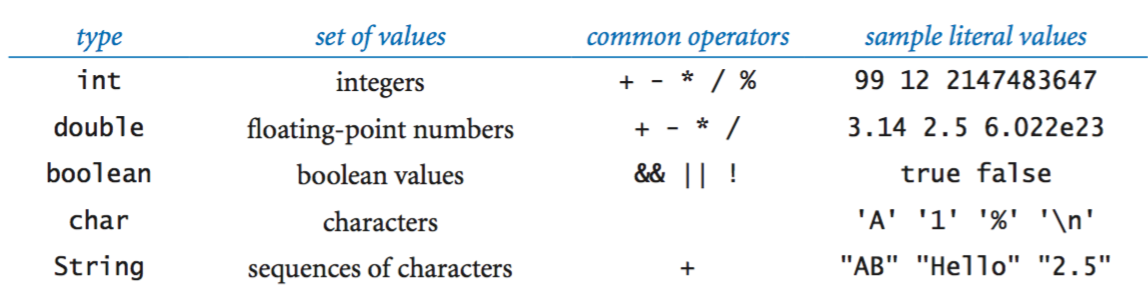
\includegraphics[width=0.85\textwidth]{images/data_types}
	\label{fig:data_types_reference}
	\caption{Types and their associated operators}
\end{figure}

Here are some examples:

\begin{code}
int n = 10;
int k = 3;
double x = 0.5;

System.out.println(n * k); 
System.out.println(n / x); 
System.out.println(n / k); // 10 = 3 * 3 + 1 
System.out.println(n % k); 
\end{code}

Output
\begin{code}
30
20.0
3
1
\end{code}

Notice that operations including a double will return a double value, even if it happens to be an integral value (like 20.0), but operations between two integers will return an integer.

The boolean operators are summarized in this table:

\begin{figure}[h]
	\centering
	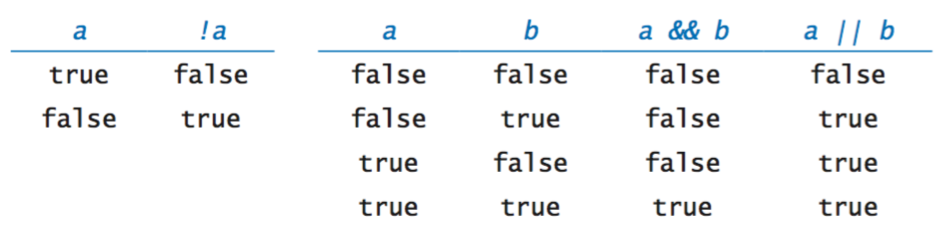
\includegraphics[width=0.85\textwidth]{images/booleans}
	\label{fig:booleans_reference}
    \caption{Boolean operators}

\end{figure}

Here's an example using boolean operators to test complex conditions:

\begin{code}
    int num = 123;
    boolean isNumEven = num % 2 == 0;
    System.out.println(isNumEven);
    boolean isNumPositive = num > 0;
    System.out.println(isNumPositive);
    System.out.println(isNumEven && isNumPositive);
    System.out.println((isNumEven && isNumPositive) || (!isNumEven));  
\end{code}

Output
\begin{code}
false
true
false
true
\end{code}

\subsection{Defining and assigning}

To define a variable of a type, write 

\begin{code}
    type varName;
\end{code}

where \textit{type} is any of the types mentioned before. The name \textit{varName} must not be used anywhere else in the same scope. To assign a value to a variable, use

\begin{code}
varName = value;
\end{code}

or define and initialize a variable with a value on the same line, with

\begin{code}
type varName = value;
\end{code}

\textit{value} must be compatible with \textit{type}. You can assign an int value to a double variable, but not the opposite. If you \emph{know} that a double value can fit in an int variable, you can use 

\begin{code}
double varName = (int) value;
\end{code}

to cast it to an int.

\subsection{String methods}

Strings have many useful methods, here is a very small subset:

\begin{code}
String s = "Hello world";
System.out.println(s.charAt(2)); // note indices start at 0
System.out.println(s.equals("hello world")); 
System.out.println(s.length()); // Note length includes spaces.
System.out.println(s.toLowerCase());  
\end{code}

output
\begin{code}
l
false
11
hello world
\end{code}


Remember that the equality operator == does not work for comparing if two strings are equal, use \textit{equals} instead.

\subsection{Math functions}

Besides the usual math operations, Java has a math library with additional methods. Here's a table of frequently used ones:


\begin{table}[h!]
\centering
\begin{tabular}{ |c|c|c| }
 \hline
 Function & Description & Example \\
 \hline
 \hline
 \ic{Math.abs(x)} & Absolute value of \ic{x} & \ic{Math.abs(-10)} equals \ic{10} \\
 \hline
 \ic{Math.pow(a, b)} & \ic{a} to the power of \ic{b} ($a^b$) & \ic{Math.pow(2, 3)} equals \ic{8} \\
 \hline
 \ic{Math.sqrt(x)} & Square root of \ic{x} & \ic{Math.sqrt(16)} equals \ic{4} \\
 \hline
\end{tabular}
\caption{A list of a few mathematical functions provided in Java}
\label{table:math_functions_reference}
\end{table}


\section{Control structures}

The general structure of an if-else statement is

\begin{code}
if (ß\textcolor{mygreen}{condition}ß) 
{
    ß\textcolor{Brown}{codeIfTrue}ß
}
else
{
    ß\textcolor{Rhodamine}{codeIfFalse}ß
}
\end{code}

Here, \textit{condition} is a boolean (for example \ic{x == 3}), and \textit{codeIfTrue}, \textit{codeIfFalse} can be codes of any number of lines. An if-else statement can include more conditions to be checked if \emph{all} the previous conditions were all false, like so:

\begin{code}
if (ß\textcolor{mygreen}{condition1}ß) 
{
    ß\textcolor{Brown}{codeIfTrue}ß
}
else if (ß\textcolor{mygreen}{condition2}ß)
{
    ß\textcolor{Red}{codeIfFalse}ß
}
...
else{
    ß\textcolor{Rhodamine}{codeIfFalse}ß
}
\end{code}

An if-else statement does not have to include an else clause. If it does not, in case of the condition not being met the code inside is just not executed and the program moves on.

\section{Loop structures}

If you know beforehand how many iterations you'd like to have, a \textit{for} loop is probably suitable:

\begin{code}
for(ß\textcolor{mygreen}{int i = 0}ß; ß\textcolor{Brown}{i < 10}ß; ß\textcolor{Rhodamine}{i++})ß {
    // do something with i
}
\end{code}

the general structure of a \textit{for} loop has an \textcolor{mygreen}{initialization}, \textcolor{Brown}{stopping condition} and \textcolor{Rhodamine}{iteration expression}. 

In the initialization, a loop variable of any type (usually \textit{int}) is defined and given initial value. The stopping condition is any boolean expression. The loop will end when the condition is false. The iteration expression changes the loop variable, usually by incrementing (\ic{i++}) or decrementing it (\ic{i-{}-}).

If you don't know how many iterations you'd like to have, but know how to check for a stopping condition, a \textit{while} loop might be more suitable:

\begin{code}
while(condition){
    // do something
}
\end{code}

A while loop stops when the condition is evaluated as false. 

\section{Methods}

Methods are first \textit{defined}, and then \textit{called}. Here's an example of a method definition and call:

\begin{code}
//naming convention: verbThenCapitalized
//examples: divideWithRemainder, flipSign, saveFile

public static void doSomething() {
    // code here
}

public static void main(String[] args) {
doSomething();
}
\end{code}

A method has a \textcolor{mygreen}{return type} and \textcolor{red}{return statement} and a parameter list with \textcolor{Brown}{types} and \textcolor{Rhodamine}{parameter names}. The return statement is optional if the return type is void. Here's an annotated example:

\begin{code}

public static ß\textcolor{mygreen}{double}ß divideTwo(ß\textcolor{Brown}{double}ß ß\textcolor{Rhodamine}{first}ß, ß\textcolor{Brown}{double}ß ß\textcolor{Rhodamine}{second}ß) {
    double result = first / second;
    ß\textcolor{red}{return second}ß;
}

public static void main(String[] args) {
    double a = 3.0;
    double b = 2.0;
    double result = divideTwo(a, b);
}

\end{code}

\section{Arrays and ArrayLists}

\subsection{Arrays}

An array can be initialized empty, or with explicit values

\begin{code}

int[] arrayOfFiveInts = new int[5];
int[] numsUpToFive = {0, 1, 2, 3, 4, 5};

\end{code}

To use or assign a value in an array, use square brackets and the index of the value. Remember that indices in an array start with 0.

\begin{code}

String[] cars = {"Volvo", "BMW", "Ford", "Mazda"};

System.out.println(cars[0]);

cars[0] = "Honda";
System.out.println(cars[0]);

\end{code}

Output
\begin{code}
Volvo
Honda
\end{code}

Arrays are very convenient to use with loops. The following code initializes an array, fills it with the numbers from 1 to 100, then computes and prints their sum:

\begin{code}

int[] numbers = new int[100];

for(int i=0; i < numbers.length; i++){
    // Note that indices start with 0
    // so the value is always one more. 
    numbers[i] = i + 1;
}

int sum = 0;
for(int i=0; i < numbers.length; i++){
    sum = sum + numbers[i];
}

System.out.println(sum);

\end{code}

Output
\begin{code}
5050
\end{code}

You can define arrays of arrays, called multidimensional arrays. For example, you can represent a 3-by-3 board with numbers in the cells like this:

\begin{code}

int[][] board = new int[3][3];
// Place the number 5 in the second row and third column
board[1][2] = 5; 

\end{code}

\subsection{ArrayLists}

An ArrayList is similar to an array, but does not have a fixed size. We can add elements to an ArrayList and delete them, changing its size. Note that to use ArrayLists in your code, you need to add the following include at the head of your file:

\begin{code}
import java.util.ArrayList;
\end{code}

In addition, an ArrayList can't store primitive types like \textit{int}, \textit{double}, and \textit{boolean}. Instead, you must use \textit{Integer}, \textit{Double} and \textit{Boolean} with them. The following code initializaes an ArrayList, fills it with the numbers from 1 to 100, then computes and prints their sum.


\begin{code}
import java.util.ArrayList;

public class Snippet{

    public static void main(String []args){
        ArrayList<Integer> numbers = new ArrayList<Integer>();

        // Numbers are added to the ArrayList, instead of assigned
        // to existing positions in an array
        for(int i=1; i <= 100; i++){
            numbers.add(i);
        }
        
        int sum = 0;
        for(int i=0; i < numbers.size(); i++){
            sum = sum + numbers.get(i);
        }
    System.out.println(sum);
    }
}
\end{code}

Output
\begin{code}
5050
\end{code}

To assign a value to an existing ArrayList index \textit{i}, use its \textit{set} method. To delete the element at index \textit{i}, use \textit{remove}, as in the following example:

\begin{code}
ArrayList<String> cars = new ArrayList<String>();

cars.add("Volvo");
cars.add("Ford");
cars.add("Mazda");
System.out.println(cars); 

cars.set(1, "Honda");
System.out.println(cars); 

cars.remove(2);
System.out.println(cars); 
\end{code}

Output
\begin{code}
[Volvo, Ford, Mazda]
[Volvo, Honda, Mazda]
[Volvo, Honda]
\end{code}


Finally, you can search an whether an ArrayList contains a value. In the case of the above Arraylist, this is what it would look like:

\begin{code}
    boolean isContained = cars.contains("Volvo"); // gets true
\end{code}

\section{Classes}

A class has a declaration, and usage (or instantiation). A declaration will include the types and names of attributes, and the class's methods. It can also include a constructor (or multiple constructors) that are called on initializing an instance of the class.

Here is a sample class declaration:

\begin{code}
public class Dog {
    // Declare but do not initialize class attributes.
    String color;
    int age;
    
    // This is a class constructor for the 'dog' class.
    public Dog(String myColor, int myAge) {
    color = myColor;
    age = myAge;
    }
    
    void bark() {
    System.out.printf("Woof! I have %s fur and %d-years-old.\n", color, age);
    }
}
\end{code}


The following code creates instances of the Dog class and uses them:

\begin{code}
public static void main(String[] args) {
    Dog fido = new Dog("brown", 3);
    Dog izzy = new Dog("black", 5);
    fido.bark();
    izzy.bark();
}
\end{code}

Output
\begin{code}
Woof! I have brown fur and 3-years-old.
Woof! I have black fur and 5-years-old.
\end{code}

To have attributes or methods that are common to the class, and not to each individual instance, use the \textit{static} modifier:

\begin{code}
public class Dog {
    private static int numDogs = 0;
    
    private static void printNumDogs(){
        System.out.println(numDogs);
    }
}
\end{code}

Note that you will usually define each class in its own file. In such a project you will usually have one central class, that uses your other classes, and your \textit{main} method will be implemented there.

